\documentclass[11pt]{article}

\usepackage[T1]{fontenc}
\usepackage[utf8]{inputenc}
\usepackage{amsmath,amssymb,amsthm}
\usepackage{graphicx}
\usepackage{booktabs}
\usepackage{siunitx}
\usepackage[margin=1.1in]{geometry}
\usepackage[colorlinks=true,linkcolor=blue,citecolor=blue,urlcolor=blue]{hyperref}

\newtheorem{definition}{Definition}
\newtheorem{proposition}{Proposition}
\theoremstyle{remark}
\newtheorem{remark}{Remark}
\newtheorem{openproblem}{Open Problem}

\title{A Computational Framework for the Composite Action of
Fundamental Physics, with a Reproduction of Gauge-Coupling Unification}
\author{Professor Codephreak\thanks{An AI-assisted project of
Gregory~L. Magnusson. Restructured in 2026 in response to an independent
academic evaluation \cite{evaluation}; code and documentation at
\url{https://github.com/GrandUnifiedTheoryOfEverything/gutoe}.}}
\date{June 2026}

\begin{document}
\maketitle

\begin{abstract}
We present a pedagogical and computational framework that organizes the
standard action functionals of fundamental physics --- the
Einstein--Hilbert action, the Dirac and Higgs actions in curved
spacetime, the Yang--Mills gauge action, and the formal loop expansion
--- into a single composite expression, and computes the piece of
unification physics that is honestly computable at this level: the
renormalization-group running of the three gauge couplings at one and
two loops, the resulting unification scale in the minimal supersymmetric
extension, and the proton-lifetime estimate it implies. The composite
action is presented as a \emph{definition} (an organizing framework),
not a theorem of unification: it is an additive juxtaposition of
separately established actions and carries no unifying dynamics. The
quantitative content is a reproduction of known results: the Standard
Model couplings miss a common intersection by $11$--$13\%$, while the
MSSM couplings unify to $0.7\%$ (two loops) at $M_{\mathrm{GUT}} \approx
1.3\times10^{16}\,$GeV with $\alpha_{\mathrm{GUT}}^{-1}\approx 25$,
yielding $\tau_p \sim 10^{35\text{--}36}$\,yr --- above the
Super-Kamiokande bound --- whereas the Standard Model near-miss scale is
excluded by four orders of magnitude. We state precisely what would be
required for a framework of this kind to rise from organized compilation
to scientific theory, and we make every number reproducible by running
the accompanying code.
\end{abstract}

\section{Introduction}

A theory of everything --- a single, internally consistent framework
containing the four fundamental interactions and all matter --- remains
one of the major unsolved problems in physics. The principal research
programs (string/M-theory, loop quantum gravity, asymptotic safety) are
mathematically demanding, mutually incompatible in their foundations,
and, to date, experimentally unconfirmed.

This project began as an AI-assisted exploration that assembled the
standard actions of fundamental physics into a composite expression and
visualized them. An independent academic evaluation \cite{evaluation}
examined that corpus and found it to be a faithful \emph{compilation} of
textbook actions but not a theory: it contained no formal apparatus, no
derivations, an internally inconsistent gravity sector, and no
falsifiable output. The present document is the response: the same
material reorganized with the formal apparatus the evaluation found
missing, the internal inconsistencies repaired by honest reframing, and
--- most importantly --- the addition of the unification computation
that any work in this area must exhibit (Section~\ref{sec:rg}).

Nothing in this paper is novel physics. The contribution is structural
and pedagogical: a single, runnable repository in which the assembled
inputs to the unification problem, the parts that can be computed, and
the precise gap to a real theory are presented together.

\section{Conventions}

Metric signature $(-,+,+,+)$; spacetime dimension four unless stated;
natural units $\hbar = c = 1$ in field-theoretic expressions.
Hypercharge is normalized by $Q = T_3 + Y$, and the GUT-normalized
$U(1)$ coupling is $\alpha_1 = \frac{5}{3}\alpha_Y$, a factor
\emph{derived} in Section~\ref{sec:embedding}. Physical constants
\cite{pdg}: $G = \SI{6.67430e-11}{m^3.kg^{-1}.s^{-2}}$,
$\hbar = \SI{1.054571817e-34}{J.s}$, and the cosmological constant
\begin{equation}
\Lambda = \SI{1.1056e-52}{m^{-2}}
\end{equation}
from Planck 2018 \cite{planck}. We record the units explicitly: a
dimensionless value for $\Lambda$ is meaningless, an error of the
pre-2026 corpus corrected here.

\section{The composite action}
\label{sec:action}

\begin{definition}[Composite action; organizing framework]
\label{def:composite}
\begin{align}
S \;&=\; S_{\mathrm{gravity}} + S_{\mathrm{matter}}
        + S_{\mathrm{gauge}} + S_{\mathrm{quantum}},\\[4pt]
S_{\mathrm{gravity}} \;&=\; \frac{1}{16\pi G}\int d^4x\,\sqrt{-g}\,
        \left(R - 2\Lambda\right),\\
S_{\mathrm{matter}} \;&=\; \int d^4x\,\sqrt{-g}\,
        \Bigl[\bar{\psi}\bigl(i\gamma^{\mu}D_{\mu}-m\bigr)\psi
        + \bigl(D_{\mu}\phi\bigr)^{\dagger}\bigl(D^{\mu}\phi\bigr)
        - V(\phi)\Bigr],\\
S_{\mathrm{gauge}} \;&=\; -\frac{1}{4}\int d^4x\,\sqrt{-g}\,
        F^{a}_{\mu\nu}F^{a\,\mu\nu},\\
S_{\mathrm{quantum}} \;&=\; \sum_{n=1}^{\infty}\hbar^{n}S_{n},
\end{align}
with $V(\phi) = -\mu^2|\phi|^2 + \lambda|\phi|^4$ ($\mu^2,\lambda>0$)
and $F^{a}_{\mu\nu} = \partial_{\mu}A^{a}_{\nu} -
\partial_{\nu}A^{a}_{\mu} + g f^{abc}A^{b}_{\mu}A^{c}_{\nu}$.
\end{definition}

Definition~\ref{def:composite} \emph{organizes} the standard actions of
fundamental physics in one expression. It is a definition, not a
theorem: the sum carries no unifying dynamics beyond that of its parts.
Each term is a transcription of an established, separately tested
action; what a genuine unification requires --- a single gauge group
from which the forces emerge, derived inter-sector couplings, a
consistent quantization --- is exactly what the bare sum does not
supply. We return to this distinction in Section~\ref{sec:open}.

\begin{remark}[The gravity sector: one action, several research
programs]
\label{rem:gravity}
Only the Einstein--Hilbert action enters $S$. The loop-quantum-gravity
(Ashtekar-variable) action and the string-theoretic (NS--NS sector)
effective action, which earlier versions of this project listed as
parallel ``formulations'' of $S_{\mathrm{gravity}}$, are mutually
exclusive candidate UV completions: they live in different dimensions
(4 vs.\ 10), are built on different fundamental variables, and belong
to competing research programs \cite{rovelli,polchinski}. They may be
compared; they may not be summed. A unified theory must select or
derive one and recover the others' regimes as limits --- a derivation
that exists neither here nor, to date, anywhere.
\end{remark}

\section{Embedding the Standard Model in SU(5) and SO(10)}
\label{sec:embedding}

This section is an exposition of known results
\cite{georgi-glashow,fritzsch-minkowski}, included because it is the
group-theoretic arithmetic any unification claim must exhibit, and
because the RG analysis of Section~\ref{sec:rg} requires the
normalization derived here. Every number is reproduced by
\texttt{python3 -m toe\_math.gut\_embedding}.

One generation of Standard Model fermions (15 left-handed Weyl spinors)
fits exactly into $\bar{\mathbf{5}}\oplus\mathbf{10}$ of SU(5)
(Table~\ref{tab:embedding}).

\begin{table}[ht]
\centering
\begin{tabular}{lccccc}
\toprule
Field & $SU(3)_c$ & $SU(2)_L$ & $Y$ & States & $SU(5)$ irrep\\
\midrule
$Q=(u_L,d_L)$ & $\mathbf{3}$ & $\mathbf{2}$ & $1/6$ & 6 & $\mathbf{10}$\\
$u^c_L$ & $\bar{\mathbf{3}}$ & $\mathbf{1}$ & $-2/3$ & 3 & $\mathbf{10}$\\
$e^c_L$ & $\mathbf{1}$ & $\mathbf{1}$ & $1$ & 1 & $\mathbf{10}$\\
$d^c_L$ & $\bar{\mathbf{3}}$ & $\mathbf{1}$ & $1/3$ & 3 & $\bar{\mathbf{5}}$\\
$L=(\nu_L,e_L)$ & $\mathbf{1}$ & $\mathbf{2}$ & $-1/2$ & 2 & $\bar{\mathbf{5}}$\\
\bottomrule
\end{tabular}
\caption{One SM generation in SU(5). Conventions: left-handed Weyl
fermions, $Q = T_3 + Y$.}
\label{tab:embedding}
\end{table}

\paragraph{The hypercharge normalization, derived.} In SU(5) all
generators are normalized identically, so $\mathrm{Tr}(T^2)$ over a
generation must agree between $T_3$ and the properly normalized
hypercharge generator. From Table~\ref{tab:embedding},
\begin{equation}
\mathrm{Tr}(Y^2) = 6\cdot\tfrac{1}{36} + 3\cdot\tfrac{4}{9} + 1
+ 3\cdot\tfrac{1}{9} + 2\cdot\tfrac{1}{4} = \tfrac{10}{3},
\qquad
\mathrm{Tr}(T_3^2) = 2,
\end{equation}
hence $T_1 = \sqrt{3/5}\,Y$ and $\alpha_1 = \frac{5}{3}\alpha_Y$.

\paragraph{Anomaly cancellation.} Within one generation the four gauge
anomaly sums vanish exactly: $\sum Y = 0$, $\sum Y^3 = 0$,
$\sum_{\mathrm{colored}} Y = 0$ ($SU(3)^2$--$U(1)$), and
$\sum_{\mathrm{doublets}} Y = 0$ ($SU(2)^2$--$U(1)$).

\paragraph{SO(10).} The spinorial $\mathbf{16}$ branches under SU(5) as
$\mathbf{16} = \mathbf{10}\oplus\bar{\mathbf{5}}\oplus\mathbf{1}$,
accommodating one generation plus a right-handed neutrino --- the
natural seed of the seesaw mechanism \cite{fritzsch-minkowski}.

\begin{proposition}[Embedding arithmetic]
\label{prop:embedding}
One SM generation fits exactly into
$\bar{\mathbf{5}}\oplus\mathbf{10}$ of SU(5); the normalization
$\alpha_1 = \frac{5}{3}\alpha_Y$ follows from
$\mathrm{Tr}(Y^2) = 10/3$; all four anomaly sums vanish; and
$\mathbf{16} = \mathbf{10}\oplus\bar{\mathbf{5}}\oplus\mathbf{1}$ under
$SO(10)\supset SU(5)$.
\emph{Proof: by computation
(\texttt{toe\_math/gut\_embedding.py}).}\qedhere
\end{proposition}

This arithmetic shows the Standard Model \emph{fits} in SU(5)/SO(10) ---
a necessary condition and the reason GUTs are taken seriously. It does
not establish unification (Section~\ref{sec:open}).

\section{Renormalization-group analysis}
\label{sec:rg}

Every number in this section is reproduced by
\texttt{python3 -m toe\_math.rg\_running}.

\subsection{Inputs and boundary conditions}

PDG 2024 world averages in the $\overline{\mathrm{MS}}$ scheme at
$\mu = M_Z = \SI{91.1876}{GeV}$ \cite{pdg}:
$\alpha_{em}^{-1}(M_Z) = 127.951$, $\sin^2\theta_W(M_Z) = 0.23122$,
$\alpha_s(M_Z) = 0.1179$. In GUT normalization,
\begin{equation}
\alpha_1^{-1} = \tfrac{3}{5}\cos^2\theta_W\,\alpha_{em}^{-1} = 59.02,
\quad
\alpha_2^{-1} = \sin^2\theta_W\,\alpha_{em}^{-1} = 29.58,
\quad
\alpha_3^{-1} = \alpha_s^{-1} = 8.48.
\end{equation}

\subsection{Running}

At one loop, $\alpha_i^{-1}(\mu) = \alpha_i^{-1}(M_Z) -
\frac{b_i}{2\pi}\ln\frac{\mu}{M_Z}$ with
\begin{equation}
b^{\mathrm{SM}} = \left(\tfrac{41}{10},\, -\tfrac{19}{6},\, -7\right),
\qquad
b^{\mathrm{MSSM}} = \left(\tfrac{33}{5},\, 1,\, -3\right).
\end{equation}
At two loops the coupled system
\begin{equation}
\frac{d\alpha_i^{-1}}{d\ln\mu} = -\frac{1}{2\pi}\Bigl[b_i
+ \frac{1}{4\pi}\sum_j b_{ij}\,\alpha_j\Bigr]
\end{equation}
is integrated numerically with the standard matrices $b_{ij}$
\cite{machacek-vaughn,martin-ramond}; Yukawa contributions are
neglected (a percent-level effect dominated by the top Yukawa). For the
MSSM, SM beta functions are used from $M_Z$ to the superpartner
threshold $m_{\mathrm{SUSY}}$ (1\,TeV unless stated) and MSSM beta
functions above it.

\subsection{Unification criterion and results}

Pairwise crossing \emph{scales} spread widely even for good
unification, because the running lines intersect at shallow angles; the
honest discriminator is the \emph{coupling-space mismatch}: the
relative deviation of $\alpha_3^{-1}$ from $\alpha_1^{-1} =
\alpha_2^{-1}$ at their crossing. We call the couplings unified when
the mismatch is below $3\%$.

\begin{figure}[ht]
\centering
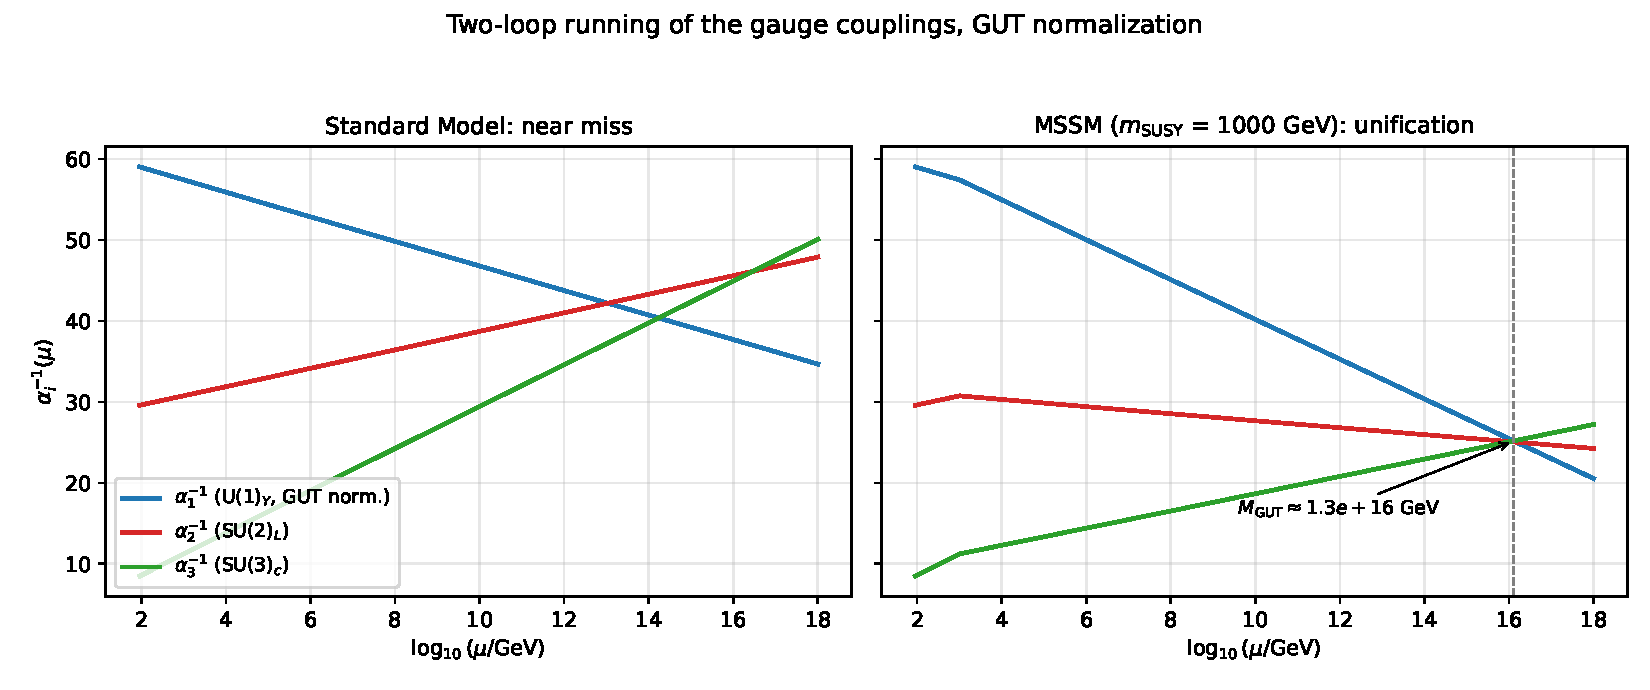
\includegraphics[width=\textwidth]{figures/rg_unification.pdf}
\caption{Two-loop running of the GUT-normalized inverse couplings.
Left: Standard Model --- the couplings approach but miss a common
point. Right: MSSM with $m_{\mathrm{SUSY}} = 1$\,TeV --- unification at
$M_{\mathrm{GUT}} \approx 1.3\times10^{16}$\,GeV. Generated by
\texttt{toe\_math/rg\_running.py}.}
\label{fig:rg}
\end{figure}

\begin{table}[ht]
\centering
\begin{tabular}{llcccc}
\toprule
Model & Loops & $M_{\mathrm{GUT}}$ [GeV] & $\alpha_{\mathrm{GUT}}^{-1}$
& Mismatch & $\tau_p$ [yr]\\
\midrule
SM   & 1 & $6.2\times10^{14}$ & 41.9 & 13.1\% & $7.5\times10^{30}$\\
MSSM & 1 & $1.5\times10^{16}$ & 25.7 & 2.3\%  & $1.0\times10^{36}$\\
SM   & 2 & $3.8\times10^{14}$ & 41.7 & 11.5\% & $1.0\times10^{30}$\\
MSSM & 2 & $1.3\times10^{16}$ & 25.1 & 0.7\%  & $4.5\times10^{35}$\\
\bottomrule
\end{tabular}
\caption{Unification analysis. $M_{\mathrm{GUT}}$ is the geometric mean
of the three pairwise crossing scales; $\tau_p$ is the dimensional
estimate of Proposition~\ref{prop:proton}.}
\label{tab:results}
\end{table}

\begin{proposition}[Standard Model near-miss]
\label{prop:sm}
With the stated inputs, the SM couplings fail to unify: at the
$\alpha_1 = \alpha_2$ crossing, $\alpha_3^{-1}$ deviates by $13.1\%$
(one loop) and $11.5\%$ (two loops) --- an order of magnitude beyond
experimental uncertainty. \emph{Proof: by computation.}
\end{proposition}

\begin{proposition}[MSSM unification]
\label{prop:mssm}
With $m_{\mathrm{SUSY}} = 1$\,TeV, the couplings unify to $2.3\%$ (one
loop) and $0.7\%$ (two loops) at $M_{\mathrm{GUT}} \approx
1.3\text{--}1.5\times10^{16}$\,GeV with
$\alpha_{\mathrm{GUT}}^{-1} \approx 25$, reproducing
\cite{amaldi,martin-ramond}. \emph{Proof: by computation.}
\end{proposition}

\section{Proton lifetime}
\label{sec:proton}

\begin{proposition}[Proton-lifetime estimate]
\label{prop:proton}
The dimensional estimate for gauge-boson-mediated $p\to e^+\pi^0$,
\begin{equation}
\tau_p \;\sim\; \frac{M_{\mathrm{GUT}}^4}
{\alpha_{\mathrm{GUT}}^2\,m_p^5},
\end{equation}
gives $\tau_p \sim 10^{35\text{--}36}$\,yr at the MSSM unification
point --- consistent with the Super-Kamiokande bound
$\tau_p > 2.4\times10^{34}$\,yr \cite{superk} --- while the SM
near-miss scale ($\sim 10^{14\text{--}15}$\,GeV) would imply $\tau_p
\sim 10^{30\text{--}31}$\,yr, excluded by four orders of magnitude.
\emph{Proof: by computation; order-of-magnitude only.}
\end{proposition}

The estimate carries $\mathcal{O}(10^{1\text{--}2})$ uncertainty from
hadronic matrix elements and thresholds; the comparison with experiment
is order-of-magnitude. The excluded SM scenario is the classic demise
of minimal non-supersymmetric SU(5) \cite{georgi-glashow,superk}.
Conversely, LHC limits (gluinos above 2.3\,TeV, squarks above 1.85\,TeV
in simplified models \cite{atlas}) pressure the
$m_{\mathrm{SUSY}} \sim 1$\,TeV assumption from below; the dependence
of Proposition~\ref{prop:mssm} on $m_{\mathrm{SUSY}}$ is logarithmic
and is exposed as an interactive parameter in the accompanying
application.

\section{Limitations and open problems}
\label{sec:open}

What would be required for this framework to rise from organized
compilation to scientific theory (after \cite{evaluation}, \S6.4):

\begin{openproblem}
A single unifying gauge group with the full three-generation dynamics
--- Yukawa sector, mixing angles, symmetry breaking --- derived, not
only the one-generation group theory of
Proposition~\ref{prop:embedding}.
\end{openproblem}

\begin{openproblem}
Derived inter-sector couplings: matter--gravity, gauge--gravity, and
scalar-sector interactions following from one principle.
\end{openproblem}

\begin{openproblem}
A cure for gravitational non-renormalizability: the two-loop divergence
of quantized Einstein gravity \cite{goroff-sagnotti,thooft-veltman}
must be addressed by a demonstrated mechanism --- finiteness (string
theory), a non-trivial fixed point (asymptotic safety), or otherwise.
The formal loop expansion $S_{\mathrm{quantum}}$ of
Definition~\ref{def:composite} presupposes exactly the consistency that
is at issue.
\end{openproblem}

\begin{openproblem}
Selection in the gravity sector: exactly one UV completion, with the
others recovered or excluded in appropriate limits
(Remark~\ref{rem:gravity}).
\end{openproblem}

\begin{openproblem}
A novel falsifiable prediction beyond those of the constituent
theories: a proton lifetime with controlled hadronic uncertainties, a
superpartner mass, or a measurable coupling deviation.
\end{openproblem}

\section{Conclusion}

This paper presents the honest version of an ambitious project. The
composite action of Definition~\ref{def:composite} organizes --- it
does not unify. The quantitative content
(Propositions~\ref{prop:embedding}--\ref{prop:proton}) is a
reproduction of the classic unification analysis, included because any
work that speaks about unification must compute what is computable at
its level, and made fully reproducible as running code. The distance
between this framework and a theory of everything is stated precisely
as Open Problems 1--5; none is solved here, and none is solved
anywhere. The project's value is pedagogical and structural: the
assembled inputs to the unification problem, the computable parts
computed, and the gap to a real theory kept in plain sight.

\begin{thebibliography}{19}

\bibitem{georgi-glashow} H.~Georgi and S.~L. Glashow, \emph{Unity of
all elementary-particle forces}, Phys. Rev. Lett. \textbf{32}, 438
(1974).

\bibitem{gqw} H.~Georgi, H.~R. Quinn, and S.~Weinberg, \emph{Hierarchy
of interactions in unified gauge theories}, Phys. Rev. Lett.
\textbf{33}, 451 (1974).

\bibitem{fritzsch-minkowski} H.~Fritzsch and P.~Minkowski,
\emph{Unified interactions of leptons and hadrons}, Ann. Phys.
\textbf{93}, 193 (1975).

\bibitem{dimopoulos-georgi} S.~Dimopoulos and H.~Georgi, \emph{Softly
broken supersymmetry and SU(5)}, Nucl. Phys. B \textbf{193}, 150
(1981).

\bibitem{amaldi} U.~Amaldi, W.~de Boer, and H.~F\"urstenau,
\emph{Comparison of grand unified theories with electroweak and strong
coupling constants measured at LEP}, Phys. Lett. B \textbf{260}, 447
(1991).

\bibitem{martin-ramond} P.~Martin and P.~Ramond, \emph{Sorting out the
minimal supersymmetric standard model}, arXiv:hep-ph/9501244.

\bibitem{martin-primer} S.~P. Martin, \emph{A supersymmetry primer},
arXiv:hep-ph/9709356.

\bibitem{machacek-vaughn} M.~E. Machacek and M.~T. Vaughn,
\emph{Two-loop renormalization group equations in a general quantum
field theory}, Nucl. Phys. B \textbf{222}, 83 (1983); \textbf{236},
221 (1984); \textbf{249}, 70 (1985).

\bibitem{goroff-sagnotti} M.~H. Goroff and A.~Sagnotti, \emph{The
ultraviolet behavior of Einstein gravity}, Nucl. Phys. B \textbf{266},
709 (1986).

\bibitem{thooft-veltman} G.~'t~Hooft and M.~Veltman, \emph{One-loop
divergencies in the theory of gravitation}, Ann. Inst. H. Poincar\'e A
\textbf{20}, 69 (1974).

\bibitem{rovelli} C.~Rovelli, \emph{Quantum Gravity}, Cambridge
University Press (2004).

\bibitem{polchinski} J.~Polchinski, \emph{String Theory}, Vols. 1--2,
Cambridge University Press (1998).

\bibitem{pdg} S.~Navas \emph{et al.} (Particle Data Group),
\emph{Review of particle physics}, Phys. Rev. D \textbf{110}, 030001
(2024).

\bibitem{superk} A.~Takenaka \emph{et al.} (Super-Kamiokande),
\emph{Search for proton decay via $p\to e^+\pi^0$ and $p\to\mu^+\pi^0$
with an enlarged fiducial volume}, Phys. Rev. D \textbf{102}, 112011
(2020), arXiv:2010.16098.

\bibitem{atlas} ATLAS Collaboration, \emph{Search for squarks and
gluinos in final states with jets and missing transverse momentum at
$\sqrt{s} = 13$ TeV (139 fb$^{-1}$)}, JHEP \textbf{02}, 143 (2021),
arXiv:2010.14293.

\bibitem{planck} N.~Aghanim \emph{et al.} (Planck), \emph{Planck 2018
results VI: Cosmological parameters}, Astron. Astrophys. \textbf{641},
A6 (2020), arXiv:1807.06209.

\bibitem{weinberg-cc} S.~Weinberg, \emph{The cosmological constant
problem}, Rev. Mod. Phys. \textbf{61}, 1 (1989).

\bibitem{peskin-schroeder} M.~E. Peskin and D.~V. Schroeder, \emph{An
Introduction to Quantum Field Theory}, Westview Press (1995).

\bibitem{evaluation} \emph{Professor Codephreak's GUToE: An Independent
Academic Evaluation of an AI-Assisted Theory of Everything} (2026), PDF
in the repository root.

\end{thebibliography}

\end{document}
